\documentclass[tikz,border=4pt]{standalone}
% Estilos compartilhados pelos diagramas dos estágios e módulos do Core.
\usetikzlibrary{arrows.meta, positioning, calc, shapes.geometric, fit}

\tikzset{
  >={Stealth[length=2.2mm]},
  bloco/.style={draw, rounded corners=2pt, minimum width=24mm, minimum height=9mm,
                align=center, font=\small, fill=blue!6},
  regpipe/.style={draw, minimum width=9mm, minimum height=48mm, align=center,
                  font=\small, fill=gray!25},
  mux/.style={draw, trapezium, trapezium angle=70, shape border rotate=90,
              minimum height=11mm, minimum width=7mm, inner sep=1pt, align=center,
              font=\scriptsize, fill=orange!15},
  ctrl/.style={draw, rounded corners=2pt, minimum width=24mm, minimum height=9mm,
               align=center, font=\small, fill=green!10},
  opcional/.style={bloco, dashed, fill=yellow!12},
  externo/.style={draw, rounded corners=2pt, minimum width=24mm, minimum height=9mm,
                  align=center, font=\small, fill=red!8},
  dado/.style={->, thick},
  sinal/.style={->, dashed},
  rotulo/.style={font=\scriptsize, midway, above, inner sep=1pt},
  titulo/.style={font=\bfseries\normalsize}
}

\begin{document}
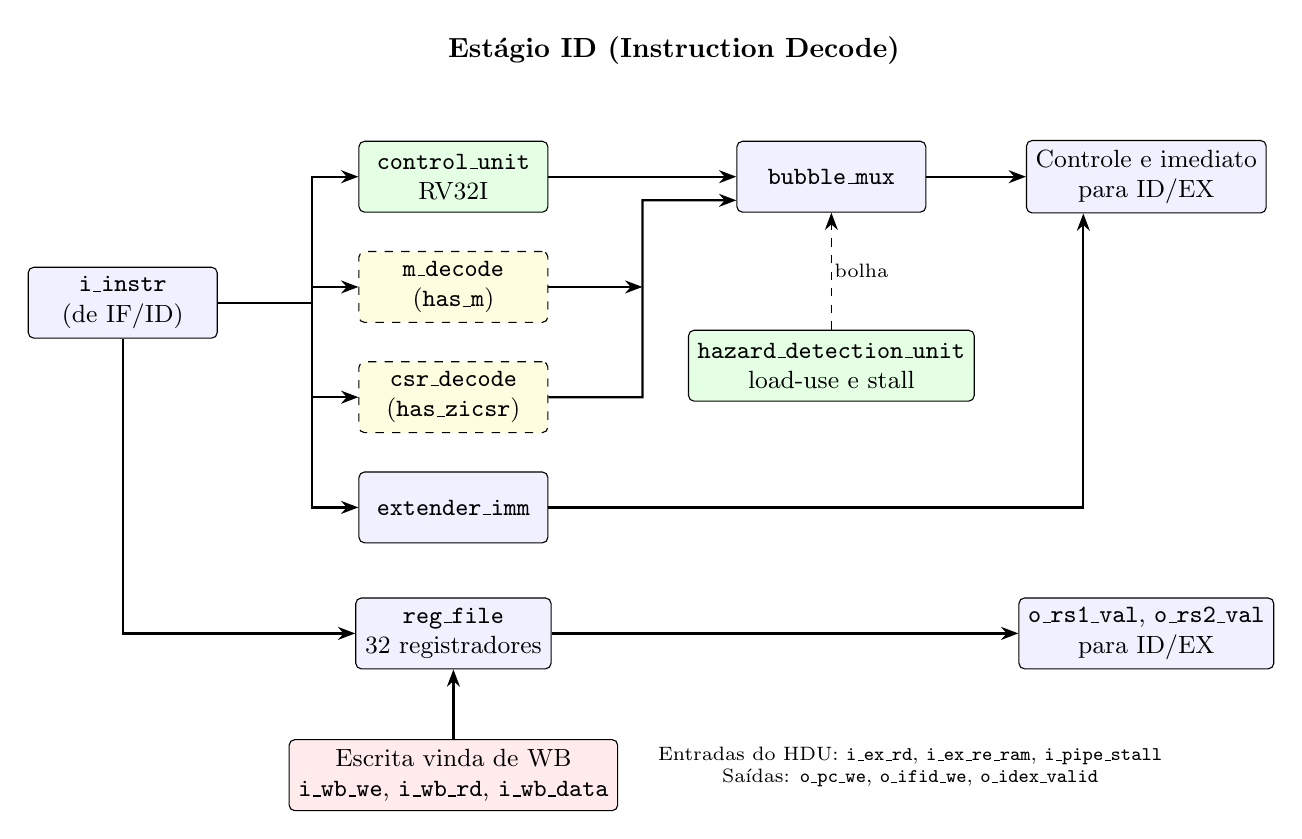
\begin{tikzpicture}
  \node[titulo] at (7,6.2) {Estágio ID (Instruction Decode)};
  \node[bloco] (instr) at (0,3) {\texttt{i\_instr}\\(de IF/ID)};
  \node[ctrl] (cu) at (4.2,4.6) {\texttt{control\_unit}\\RV32I};
  \node[opcional] (md) at (4.2,3.2) {\texttt{m\_decode}\\(\texttt{has\_m})};
  \node[opcional] (cd) at (4.2,1.8) {\texttt{csr\_decode}\\(\texttt{has\_zicsr})};
  \node[bloco] (ext) at (4.2,0.4) {\texttt{extender\_imm}};
  \node[bloco] (rf) at (4.2,-1.2) {\texttt{reg\_file}\\32 registradores};
  \node[externo] (wb) at (4.2,-3.0) {Escrita vinda de WB\\\texttt{i\_wb\_we}, \texttt{i\_wb\_rd}, \texttt{i\_wb\_data}};
  \node[bloco] (bub) at (9,4.6) {\texttt{bubble\_mux}};
  \node[ctrl] (hdu) at (9,2.2) {\texttt{hazard\_detection\_unit}\\load-use e stall};
  \node[bloco] (out) at (13,4.6) {Controle e imediato\\para ID/EX};
  \node[bloco] (outr) at (13,-1.2) {\texttt{o\_rs1\_val}, \texttt{o\_rs2\_val}\\para ID/EX};

  \draw[dado] (instr.east) -- ++(1.2,0) |- (cu.west);
  \draw[dado] (instr.east) -- ++(1.2,0) |- (md.west);
  \draw[dado] (instr.east) -- ++(1.2,0) |- (cd.west);
  \draw[dado] (instr.east) -- ++(1.2,0) |- (ext.west);
  \draw[dado] (instr.south) |- (rf.west);
  \draw[dado] (wb) -- (rf);
  \draw[dado] (cu) -- (bub);
  \draw[dado] (md.east) -- (6.6,3.2);
  \draw[dado] (cd.east) -- (6.6,1.8) -- (6.6,4.3) -- ([yshift=-3mm]bub.west);
  \draw[dado] (bub) -- (out);
  \draw[dado] (ext.east) -| ([xshift=-8mm]out.south);
  \draw[dado] (rf) -- (outr);
  \draw[sinal] (hdu) -- node[rotulo, right] {bolha} (bub);
  \node[font=\scriptsize, align=center] at (10,-2.9) {Entradas do HDU: \texttt{i\_ex\_rd}, \texttt{i\_ex\_re\_ram}, \texttt{i\_pipe\_stall}\\Saídas: \texttt{o\_pc\_we}, \texttt{o\_ifid\_we}, \texttt{o\_idex\_valid}};
\end{tikzpicture}
\end{document}
